\chapter{\IfLanguageName{dutch}{Ontwikkeling en Training van Objectdetectiemodellen}{Datacollection and Labeling}}%
\label{ch:objectdetectie}

\subsection{Doelstelling}
Deze fase was gericht op het ontwikkelen en trainen van geavanceerde objectdetectiemodellen om koeien en hun gedragingen nauwkeurig te identificeren binnen diverse agrarische omgevingen.

\subsection{Methoden}
\begin{itemize}
  \item \textbf{Voorbereiding van Data:}  De data geëxtraheerd uit Labelbox werd omgezet naar het YOLO dataformaat, wat noodzakelijk was om compatibiliteit met het modeltrainingsproces te verzekeren.
  \item \textbf{Modelselectie en Training:} Begonnen werd met het testen van verschillende YOLO-modellen. Er werd een voorgetraind YOLO-model gebruikt, gebaseerd op de COCO-dataset, om het trainingsproces te versnellen. 
  Deze modellen werden getraind op een rekencomputer uitgerust met 2 Nvidia A5000 GPU's van 25GB, wat een krachtige verwerkingscapaciteit bood voor het trainen van diepe neurale netwerken.
  Daarnaast werden een Faster R-CNN-model via Detectron en een SSD-model getest. Echter, het werd snel duidelijk dat YOLO-modellen eenvoudiger te gebruiken en op te zetten waren vanwege hun lagere complexiteit en eenvoudige implementatie. Bovendien leverden ze betere resultaten op dankzij de grote, voorgetrainde modellen die specifiek gericht zijn op objectdetectie, wat het hertrainen op aangepaste labels vergemakkelijkte.
  \item \textbf{Verfijning en Optimalisatie:} De focus verschoof naar verdere verfijning van de YOLO-modellen door verschillende parameters aan te passen en verschillende versies van YOLO te testen om de optimale configuratie te vinden voor de best mogelijke resultaten.
\end{itemize}

\subsection{Resultaten}
\begin{itemize}
  \item \textbf{Gekozen Model:}   Uiteindelijk werd gekozen om verder te gaan met het YOLO-model als de primaire keuze voor objectdetectie in dit onderzoek. Dit besluit was gebaseerd op de superieure prestaties en gebruiksgemak van het model in vergelijking met andere geteste modellen.
  \item 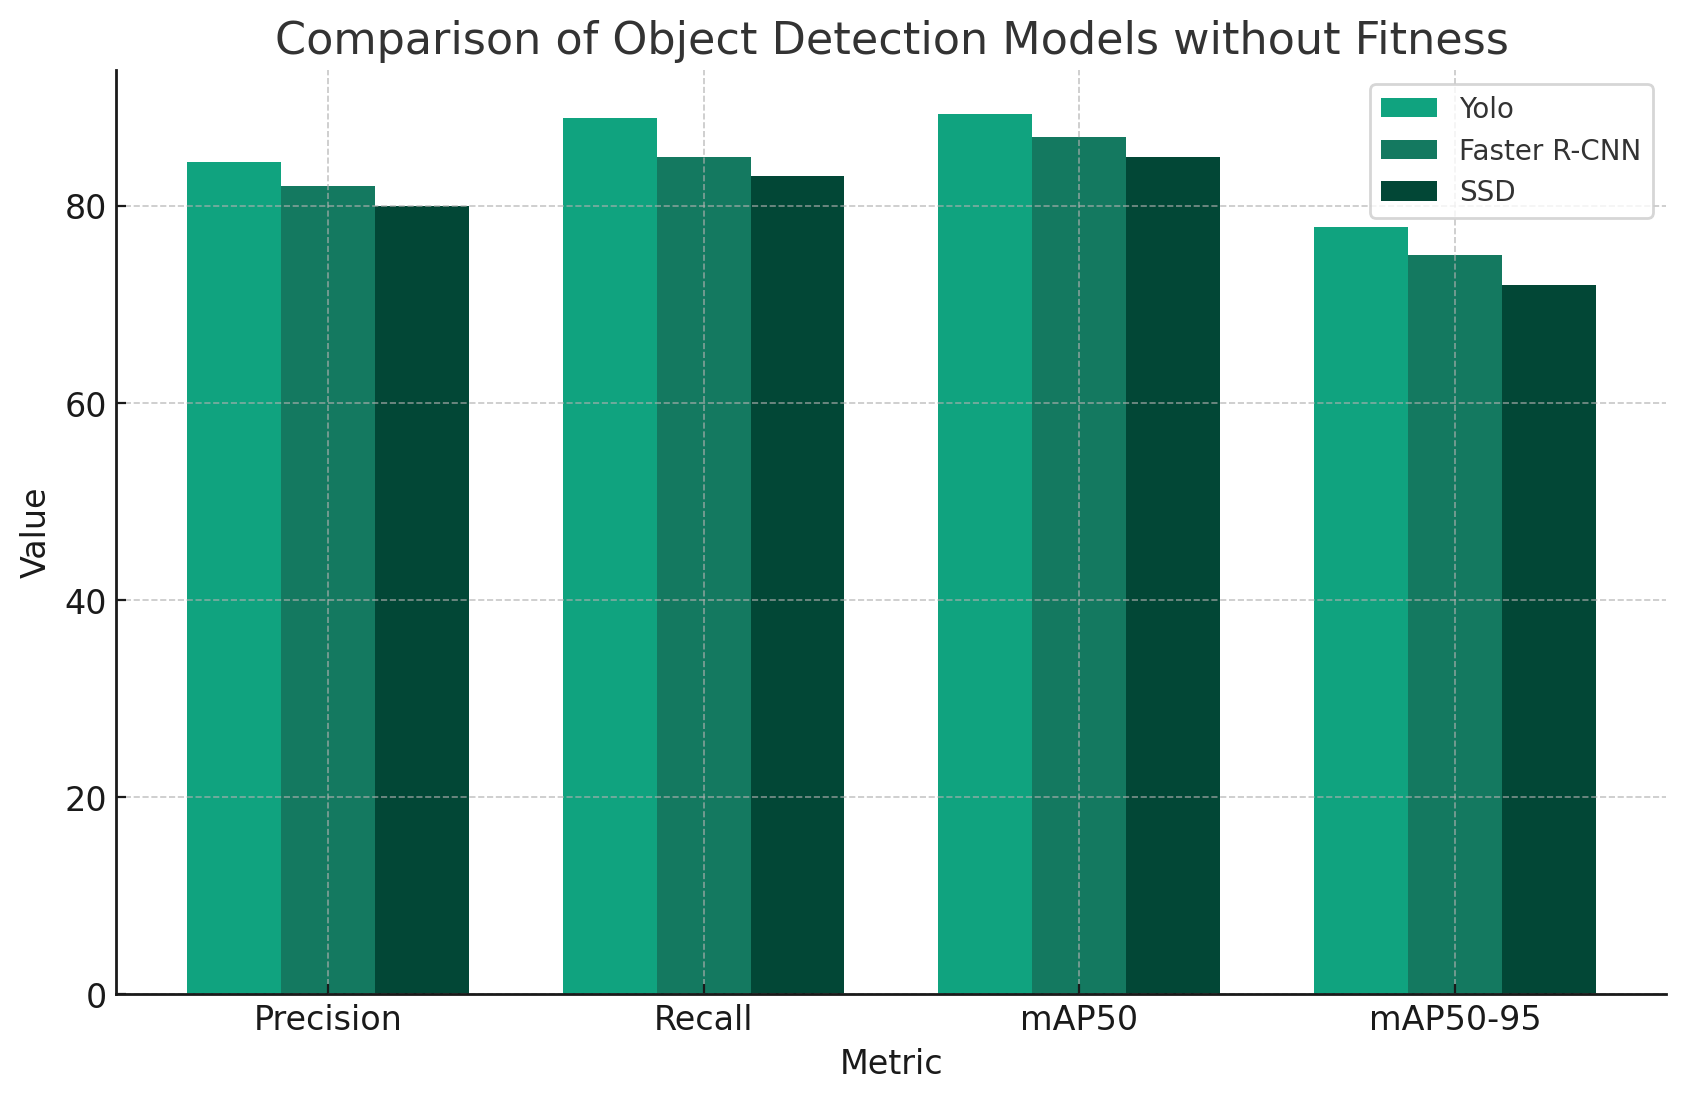
\includegraphics[width=\linewidth]{objectdetectie_metrics.png}
  \item \textbf{Modelprestaties:} Het geoptimaliseerde YOLO-model toonde duidelijke verbeteringen in het nauwkeurig detecteren en classificeren van koeiengedragingen, wat een robuust systeem opleverde dat effectief functioneerde binnen de complexe dynamiek van agrarische omgevingen.
\end{itemize}
\newline
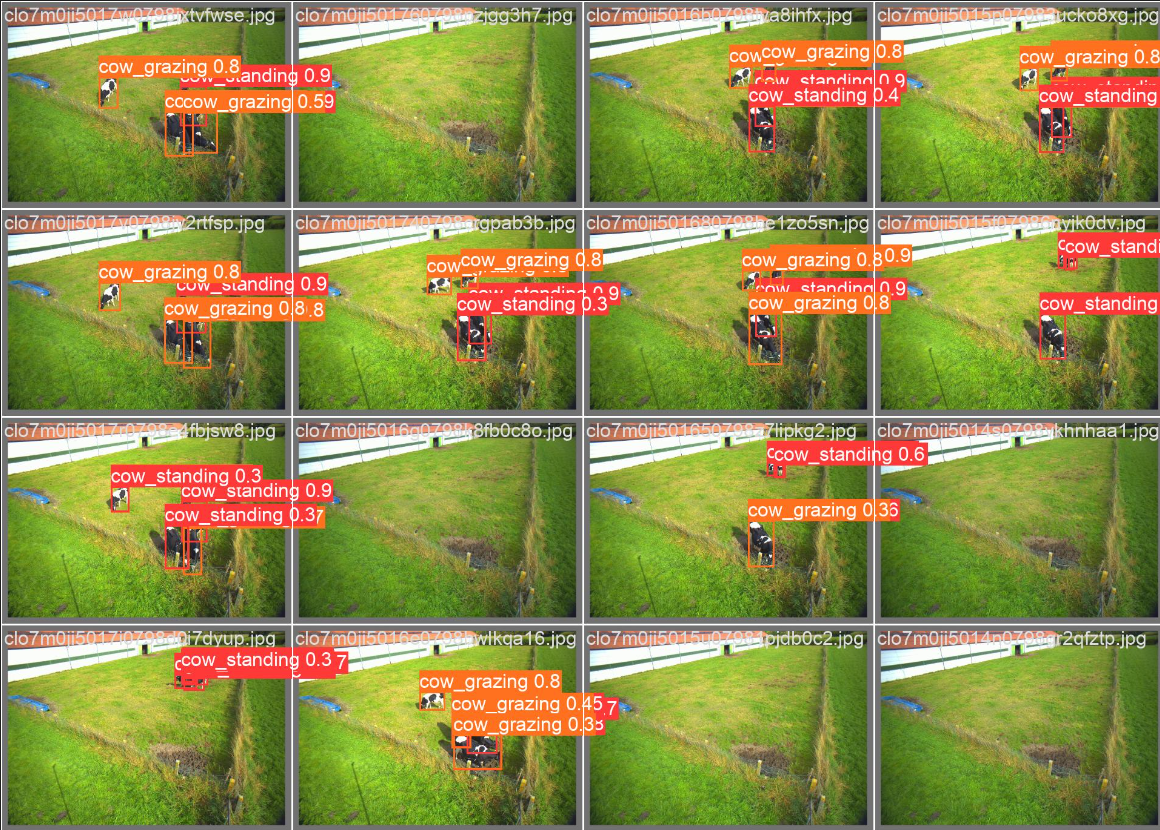
\includegraphics[width=\linewidth]{objectdetectie_yolo.png}
\newline